\documentclass[aspectratio=169]{beamer}
\usepackage[utf8]{inputenc}
\usepackage[brazil]{babel}
\usepackage{multimedia,amsmath,graphicx,color,multicol,fancyhdr,amssymb,amsfonts,amsthm,setspace}
\usepackage{ragged2e}
\usetheme{Berlin}
\usecolortheme{dolphin}
\usepackage{setspace}
\usepackage{xcolor}


% Informações que serão inseridas no slide da capa:
\title[CETi Gilberto Mestrinho]{Revisão - PSC 3}
%\author[Prof. Joao Victor]{Prof. Joao Victor}
%\institute[IFAM]{Instituto Federal do Amazonas}
\date{\today}
%\logo{
\includegraphics[scale=0.05]{logo-utfpr.png}} 

\newif\ifusarcorvermelha
\usarcorvermelhatrue % Ativa o texto vermelho (comente para desativar)

% --- Comando \vermelho ---
\newcommand{\vermelho}[1]{%
    \ifusarcorvermelha
        {\color{red}#1}% % Texto vermelho se \ifusarcorvermelha = true
    \else
        #1% % Texto normal se \ifusarcorvermelha = false
    \fi
}

\begin{document}
\justifying
\onehalfspacing


\begin{frame}
    \titlepage
\end{frame}

\section{Conteúdo Programático}

\begin{frame}{Conteúdo Programático - PSC 3}

    \begin{center}
        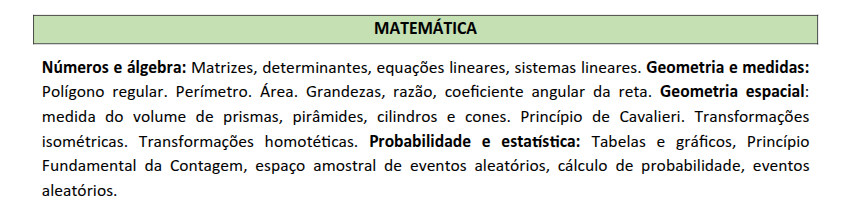
\includegraphics[scale=0.5]{PSC3.png}
    \end{center}
    
\end{frame}

\section{Questões PSC 3}

    \begin{frame}{PSC 3 - 2024 (Questão 47)}
        Estudos demográficos revelam que a população de certo país, no ano zero, é $f_{0}$ e, decorridos $t$ anos, a população poderá ser estimada pela função: $f(t)=f_{0} \times  e^{0,05 . t}$. Considerando $\ln{3}=1,10$, podemos afirmar que a população desse país deverá triplicar quando decorrerem, aproximadamente,

            \begin{enumerate}[a]
                \item 10 anos.
                \item 16 anos.
                \item 18 anos.
                \item 20 anos.
                \item \vermelho{22 anos.} %
            \end{enumerate}
            
    \end{frame}


    \begin{frame}{PSC 3 - 2024 (Questão 48)}
        Seja a função $f: \mathbb{R} \to \mathbb{R}$, definida por $f(x)=9^{x+1}$. O valor de $x$, de modo que $f(4-x)=3f(x)$, deve ser:
        
            \begin{enumerate}[a]
                \item {3}/{4}
                \item {5}/{4}
                \item \vermelho{{7}/{4}} %
                \item {5}/{6}
                \item {7}/{6}
            \end{enumerate}
            
    \end{frame}

    \begin{frame}{PSC 3 - 2024 (Questão 49)}
        A tabela de distribuição de frequências, ao lado, representa o salário semanal de 37 parceiros de uma empresa. A partir dessas informações, podemos afirmar que os valores da média aproximada, da moda e da mediana são, respectivamente,

        \begin{columns}
            \begin{column}{0.3\textwidth}
                \begin{enumerate}[a]
                    \item \vermelho{371,76, 345 e 375.} %
                    \item 373,74, 315 e 345.
                    \item 374,84, 345 e 315.
                    \item 375,93, 375 e 405.
                    \item 376,96, 375 e 435.
                \end{enumerate}
            \end{column}

            \begin{column}{0.6\textwidth}
                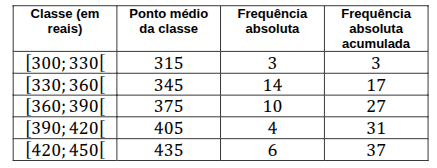
\includegraphics[width=\linewidth]{PSC2024Q49.png}
            \end{column}
        \end{columns}
                
    \end{frame}
   
\end{document}